\part{Distance control}
\chapter{Modelling}
\section{Disturbance Models}
\subsection{Aerodynamic Drag Force}
The satellite is subjected to an aerodynamic drag force due to the atmosphere. The collisions with the air caused a force in the opposite direction of the velocity of the satellite. The force was modeled by Lord Rayleigh[ref]:
%
\begin{flalign}
\vec{F_D} = \frac{1}{2} \rho \cdot C_D \cdot A_{\perp} ||\vec{v}|| \vec{v}
	\label{eq:ec1}
\end{flalign}
where $\rho$ is the density of the air, $C_D$ is the drag coefficient, $A_{\perp}$ is the area that is perpendicular of the velocity of the satellite $\vec{v}$. 

The drag coefficient $C_D$ and the perpendicular area $A_{\perp}$ depend on the orientation of the satellite. Therefore, this force can be used as an input for the control of the position and the velocity of the satellite. 

The density of the air depends on the altitude of the satellite, of the air temperature but we considered to be constant in our case to simplify the modelization. $\rho$ is chosen to be equal to $1.454 \cdot 10^-13$ $[\frac{Kg}{m^3}]$ based to the  empirical model of the Committee on Space Research (COSPAR) International Reference Atmosphere [Ref]. %J. R. Wertz, Spacecraft Attitude Determination and Control. Kluwer Academic Publishers, 1st ed., 1994.

The drag coefficient as said before is orientation dependent. The maximum value of $C_D$ is equal to 1.05 for a non tilted cubed as shown on the figure \ref{drag_coef} and equal to 0.80 for an angled cubed. In our modelization, we will assume that the drag coefficient is constant and equal to 1(not sure which value take) in order to simplified the equation. \\
\begin{table}[H]
	\begin{minipage}[b]{0.49\linewidth}
		\centering
		\begin{figure}[H]
			\centering
			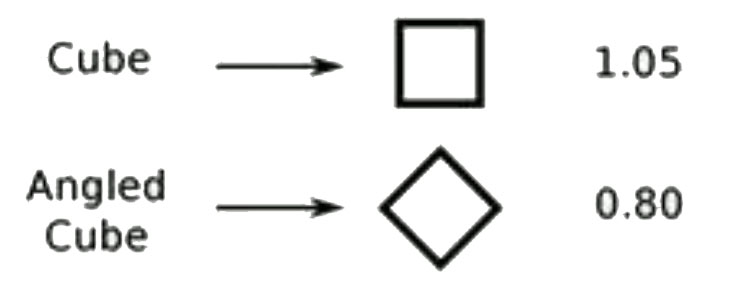
\includegraphics[width=0.7\linewidth]{figures/drag_coef}
			\caption{description needed}
			\label{fig:des1}
		\end{figure}
	\end{minipage}\hfill
	\begin{minipage}[b]{0.49\linewidth}
		\centering
		\begin{figure}[H]
			\centering
			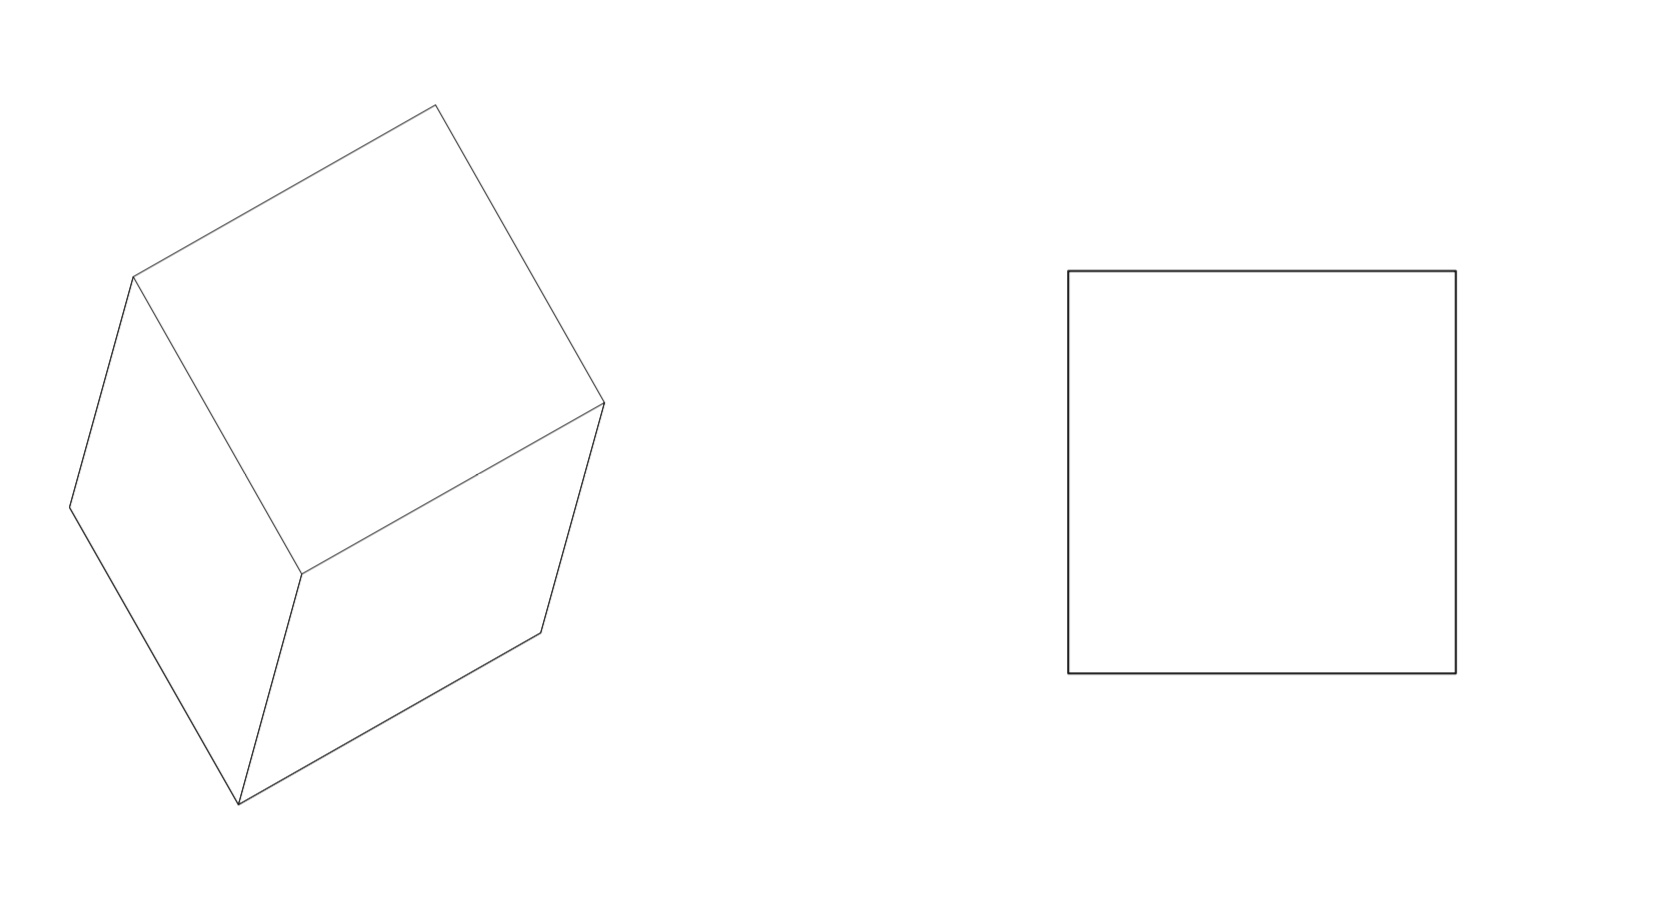
\includegraphics[width=1\linewidth]{figures/a_prep}
			\caption{description needed}
			\label{fig:des2}
		\end{figure}
	\end{minipage}
\end{table}
Therefore, the only parameter that we control is the perpendicular area $A_{\perp}$. The maximum and minimum value of $A_{perp}$ are represented at the figure\ref{a_perp}. Thus, the minimum value is the surface of a square of 10cm of dimension ($A_{\perp} = 100cm^2$) and the maximum value is the surface of an hexagone of 10cm of dimension ($A_{\perp} = \frac{3\sqrt{3}}{2} 100cm^2$)
%
\chapter{Distance control design}